\begin{center}
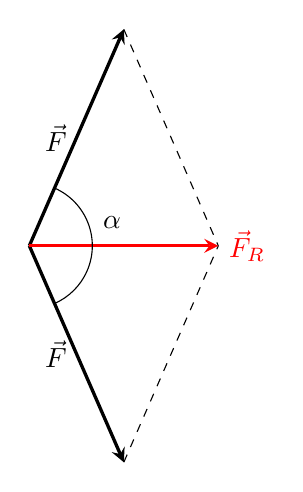
\begin{tikzpicture}[>=stealth]
 \draw[->, very thick] (0,0) -- (1.2,2.749);
 \node[left] at (0.6,1.37) {$\vec F$};
 \draw[->, very thick] (0,0) -- (1.2,-2.749);
 \node[left] at (0.6,-1.37) {$\vec F$};
 \draw[dashed] (1.2,2.749) -- (2.4,0);
 \draw[dashed] (1.2,-2.749) -- (2.4,0);
 \draw[->, very thick, red] (0,0) -- (2.4,0) node[right] {$\vec F_\text{R}$};
 \draw (0.32,0.733) arc (66.4:-66.4:0.8);
 \node at (1.05,0.3) {$\alpha$};
\end{tikzpicture}
\end{center}

Das Kräfteparallelogramm zweier gleich grosser Kräfte ist ein Rhombus, dessen Diagonale $\vec F_\text{R}$ den Winkel $\alpha$ halbiert. Daher gilt
\begin{align}
 F_\text{R} &= 2\,F\cos\frac{\alpha}{2}
\end{align}
und für den Winkel
\begin{align}
 \alpha &= \alWF \\
   &= 2\cdot\arccos\frac{\FRw}{2\cdot\Fje} \\
   &= \alW \approx \result{\alWP{0}{3}}
\end{align}
Die Resultierende ist kleiner als jede der beiden Kräfte, deshalb ist der Winkel stumpf.
